\def\difficulty{3}
\sujet{Watershed}\index{Mathematical Morphology!Watershed}
\index{Segmentation!Watershed}

\begin{note}This tutorial aims to study the watershed transform for image segmentation. 
In image processing, an image can be considered as a topographic surface. If we flood this surface from its minima and if we prevent the merging of the water coming from different sources, we partition the image into two different sets: the catchment basins separated by the watershed lines. 
\end{note}

\noindent The different processes will be applied on the following images:

\begin{figure}[h]
\begin{center}
\subfloat[circles]{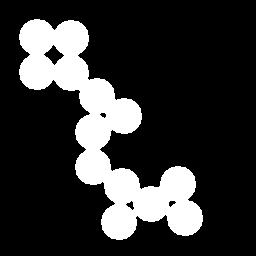
\includegraphics[width=4cm]{circles.jpg}}
\hspace*{0.025cm}
\subfloat[gel]{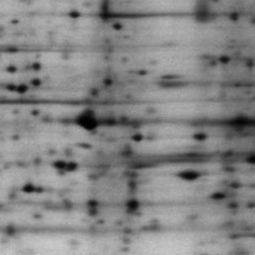
\includegraphics[width=4cm]{gel.jpg}}
\end{center}
\vspace*{-12pt}
\end{figure}

\vspace*{-10pt}


\section{Watershed and distance maps}\index{Segmentation!Distance Map}
The objective is to individualize the disks by disconnecting them with the distance map.
\begin{qbox}
\begin{itemize}
	\item Calculate the distance map of the image 'circles'.
	\item Take the complementary of this distance map and visualize its minima.
	\item Calculate the watershed transform of the inverted distance map.
	\item Subtract the watershed lines to the original image. 
\end{itemize}
\end{qbox}

\begin{mcomment}
\begin{mremark}
The distance map can be calculated by \minline{bwdist} on a binary image, the local minima are evaluated by \minline{imregionalmin}.
\end{mremark}
\end{mcomment}

\begin{pcomment}
\begin{premark}
Look at the documentation of \pinline{scipy.ndimage.morphology} for Euclidean or Chamfer distance transform. Reconstruction operator can be found in \pinline{skimage.morphology}.
\end{premark}
\end{pcomment}



\section{Watershed and image gradients}
\begin{qbox}
\begin{itemize}
	\item Calculate the Sobel gradient of the image 'gel'.
	\item Visualize the minima of the image gradient.
    \item Apply the watershed transform on the gradient image.
\end{itemize}
\end{qbox}

\noindent The watershed transform, applied in a direct way, leads to an over-segmentation. To overcome this limitation, the watershed operator can be applied on a filtered image.

\begin{qbox}
\begin{itemize}
\item Smooth the original image with a low pass filter. To stay in the mathematical morphology field, you can use an alternate morphological filter (opening followed by closing). A Gaussian filter is also a good solution.
	\item Calculate the gradient operator on the filtered image.
	\item Calculate the corresponding watershed.
\end{itemize}
\end{qbox}

\begin{mcomment}
\begin{mremark}
The mathematical morphology function of opening and closing are \minline{imopen} and \minline{imclose}.
\end{mremark}
\end{mcomment}

\section{Constrained watershed by markers}\index{Segmentation!Watershed by Markers}
In order to indivudualize the image spots, we have to determine the internal and external markers for the constrained watershed.
\begin{qbox}
\begin{itemize}
  \item Calculate the gradient (Sobel) of the filtered image.
	\item Calculate the internal markers (minima of the filtered image) and external (watershed of the filtered image) as minima of the gradient image.
	\item Calculate the corresponding watershed.
	\item Superimpose the watershed lines of the resulting segmentation to the original image.
\end{itemize}
\end{qbox}

\begin{mcomment}
\begin{mremark}
 \minline{imgradient} returns the gradient magnitude of an image. \minline{imimposemin} is used to impose minima to an image in order to perform watershed segmentation.
\end{mremark}
\end{mcomment}
